\textbf{Grünkörper} (fein/grobkörniges Metall/Keramikpulver) wird durch 
Wärmebehandlung zu einem festen Werkstück gesintert.\\
Gesinterte Teile sind deshalb nicht homogen (im Gegensatz zu 
Metalllegierungen) und können eine \textbf{Porosität} aufweisen. Diese lässt 
sich durch Kompaktieren modifizieren.\\
Durch Sintern lassen sich Stoffe zusammenbringen die auf andere 
Weise schwer oder nicht vereinbar sind.\\
Die Pulverzusammensetzung kann während des Sinterns verändert werden.\\

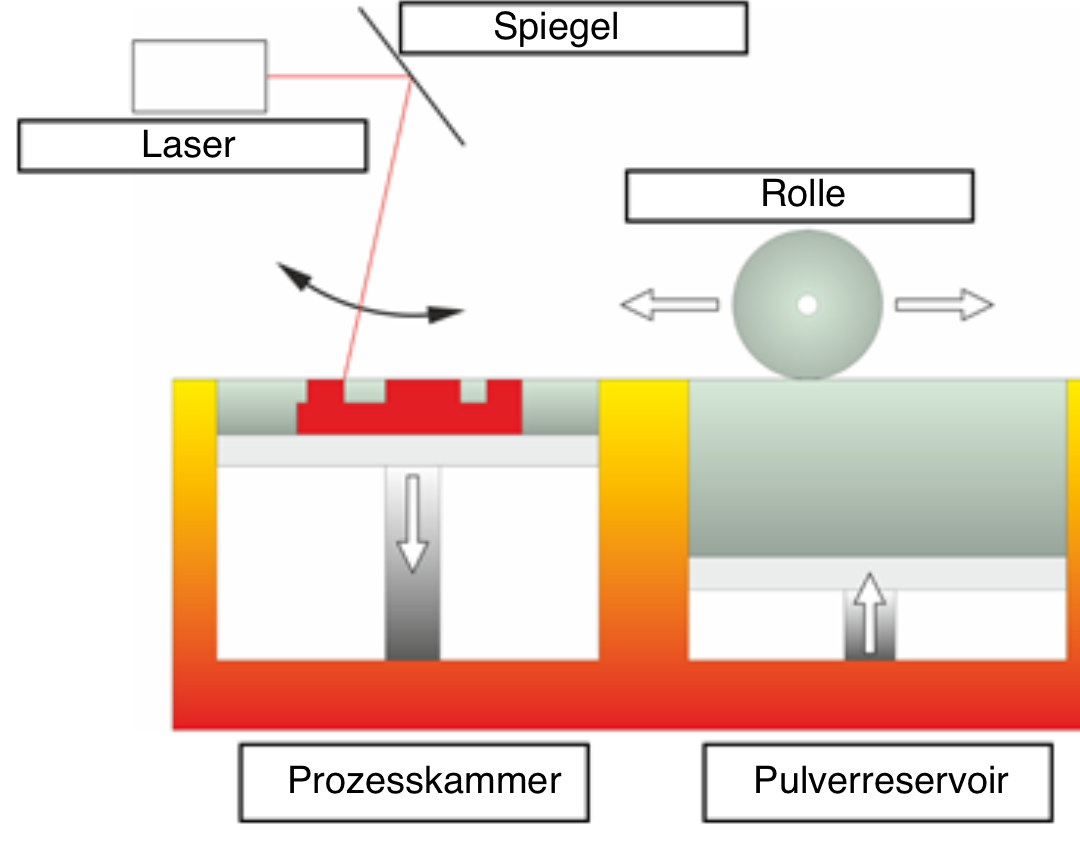
\includegraphics[width =0.6\linewidth]{src/images/Sintern.png}\\
